\section{Introduction}
The rapid advance of LLMs has positioned them as valuable tools for a wide range of decision-making tasks, including but not limited to personal assistants~\citep{liu2024dellma}, recommendation systems~\citep{li2023large}, game-playing~\citep{wang2023voyager, wang2023describe}, education~\citep{nie2024gpt, he2024evaluating}, and healthcare~\citep{singhal2023large}. 
In these tasks, LLMs function as agents that engage with users or the environment in a dynamic interaction process. For example, at each time step, the LLM suggests a pedagogical strategy or make a recommendation to a specific user, then receives feedback - either explicit or implicit - in the form of rewards. Based on this feedback, the agent updates its beliefs about the environment, e.g., underlying reward distributions, and adapts its strategies to maximize the cumulative reward. 
These tasks differ fundamentally from classic prediction tasks where LLM is used to predict a target. A decision making LLM only receives partial feedback, i.e., the reward for its own actions, but not for others. Thus, it requires the LLM to effectively interact with the environment and \emph{explore} to discover the optimal action. Meanwhile, exploring an unknown action that turns out to have lower reward than the known ones incurs an opportunity cost. The agent, therefore, needs to strike a balance between exploration and exploitation.
While the exploration-exploitation tradeoff has been extensively studied in the pre-LLM era, particularly in the fields of bandits~\citep{li2010contextual, slivkins2019introduction} and reinforcement learning~\citep{mnih2013playing,osband2013more,sutton2018reinforcement}, it remains unclear how LLMs approach this tradeoff when faced with uncertainty. 

We study LLMs' \emph{in-context exploration} capabilities under the simplified framework of bandits — a stateless form of reinforcement learning that is highly applicable to many domains. 
We set up the LLM to interact with the environment over $T$ rounds. In each round, it receives the full history of its past interactions, the current state (if provided), and a set of actions, and it is tasked with selecting an action to maximize the cumulative reward. 
Ideally, the LLM should adaptively choose an action in each round to learn the reward distributions of different actions and eventually converge to consistently selecting the optimal one. 
We study LLM's ability to do so \emph{in-context}, without the need to re-train, which we dubbed as  \emph{in-context exploration}. Unlike using LLM for reward-free or curiosity-driven exploration, \ice is in-context self-improvement, where the LLM builds up context through interactions to solve a task.

We introduce \emph{BanditBench}\footnote{Install the library: \texttt{pip install banditbench}}, a comprehensive suite of multi-armed bandit (MAB)~\citep{slivkins2019introduction} and contextual bandit (CB)~\citep{li2010contextual} environments \emph{in natural language} to rigorously evaluate the decision-making capabilities of LLMs. Building on the pioneering work of \citet{krishnamurthy2024can}, we significantly expand the benchmark by incorporating a broader range of tasks with varying complexities, including variations in the number of arms, reward distributions, exploration difficulty, and textual descriptions of environments. Additionally, we extend it to CB environments, where rewards across arms depend on contextual features, to assess generalization in LLM exploration. 

\begin{figure}[t]
    \centering
    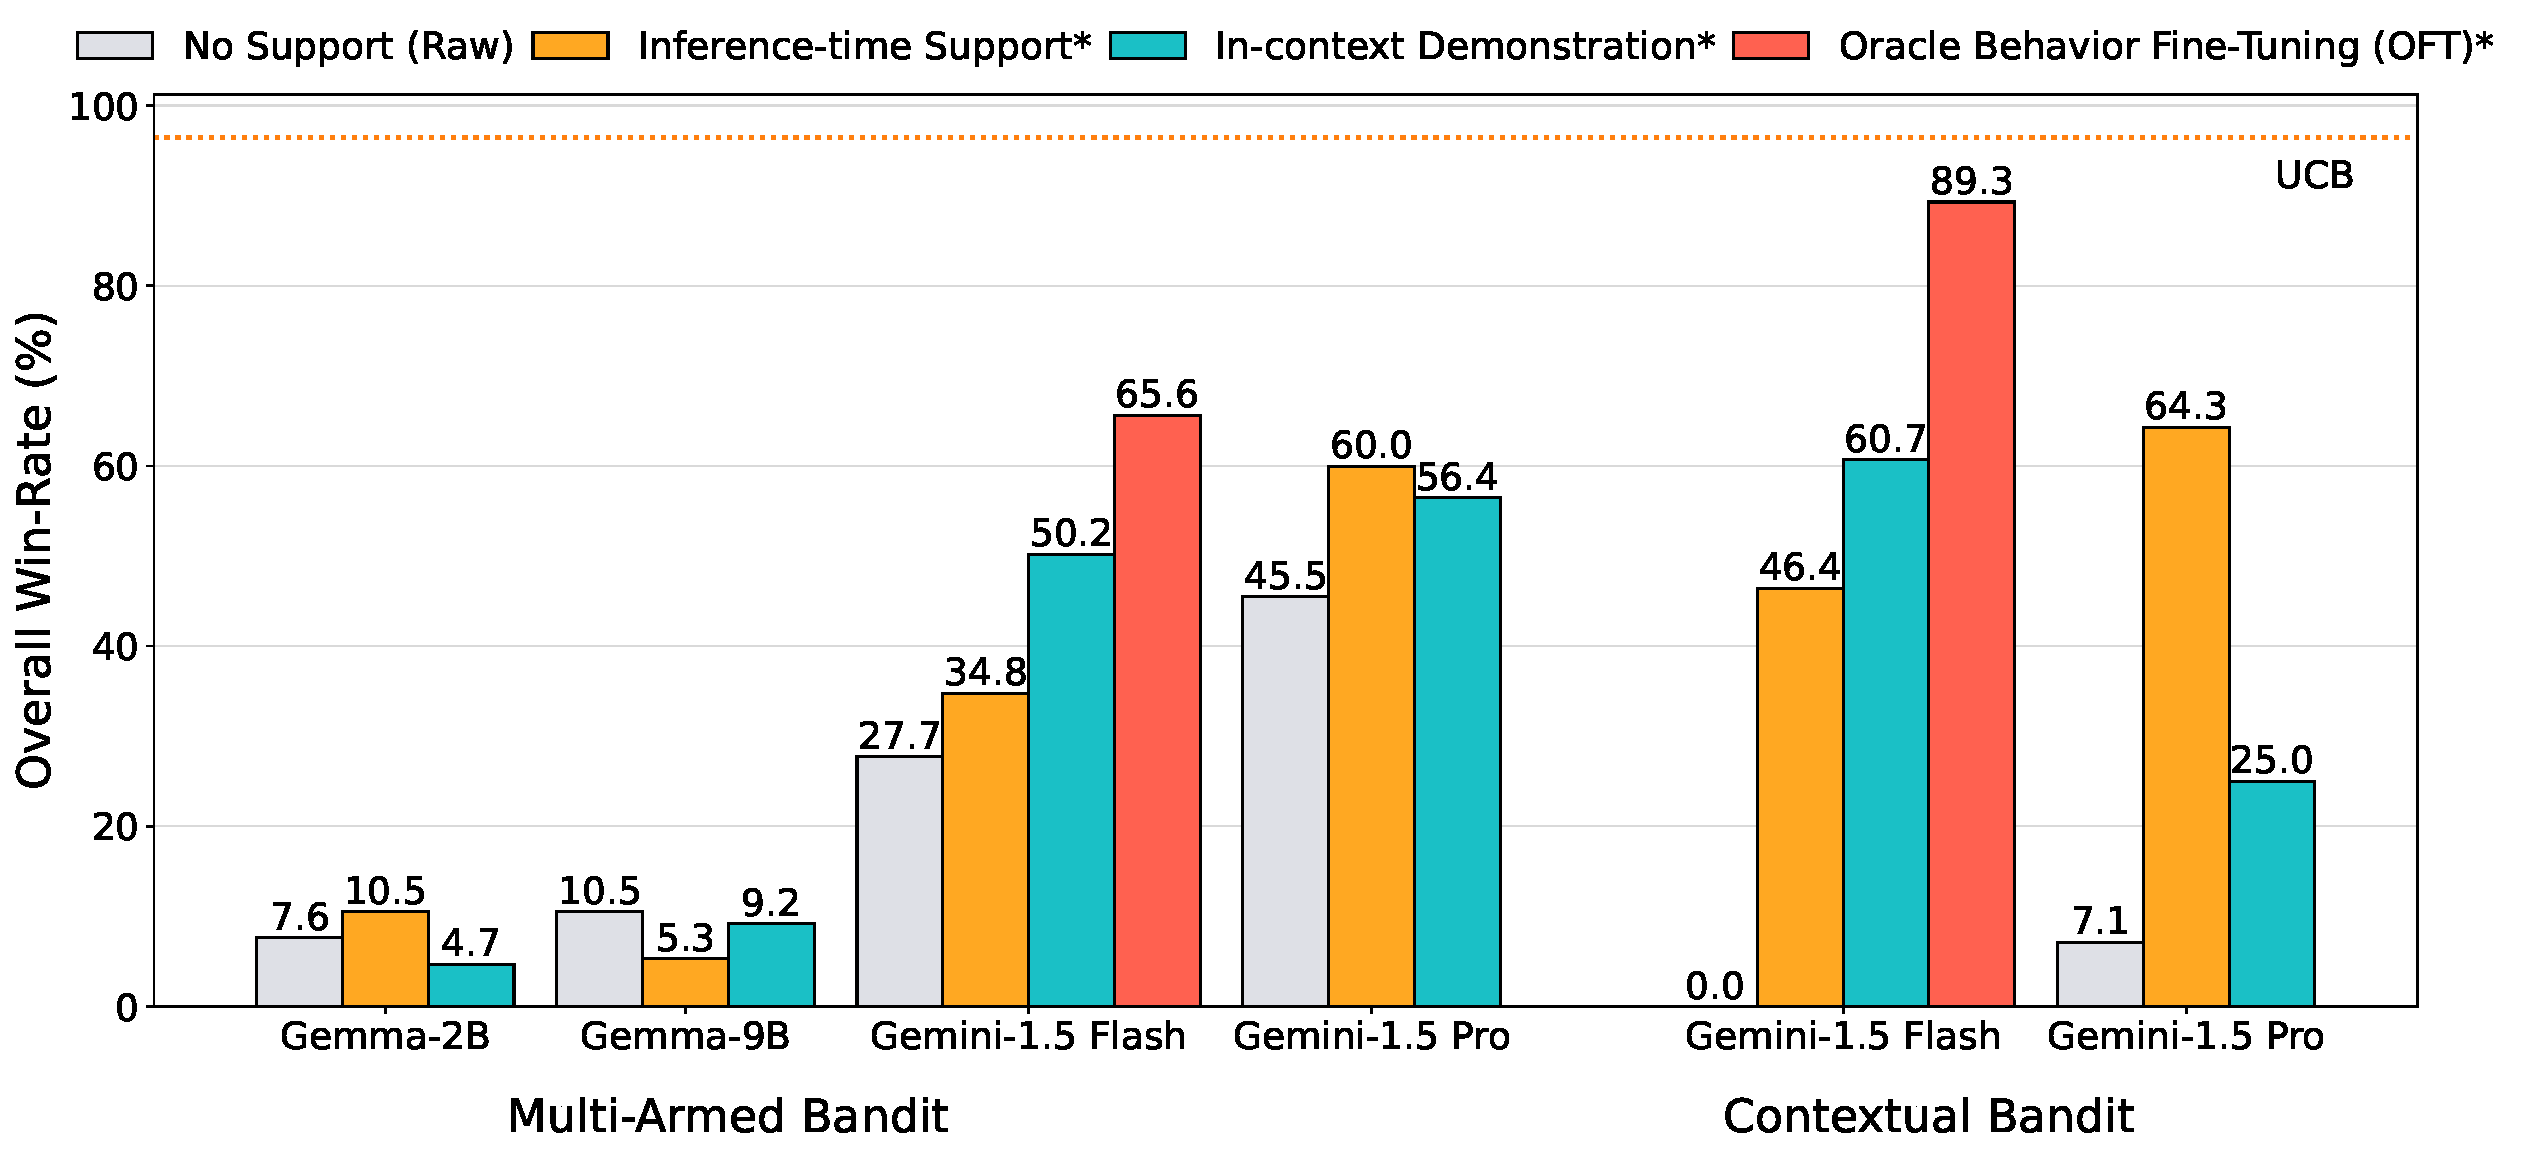
\includegraphics[width=0.9\textwidth]{figures/sft_fewshot.pdf}
    \caption{\footnotesize{The best achieved performance within each category of method in both MAB and CB. Note that we took the $\max$ over different methodology setups within each category. For contextual bandit, \OFT enabled a small fine-tuned model (Gemini-1.5 Flash) to approach the performance of the optimal classical algorithm (UCB).}}
    \label{fig:fewshot_sft_result}
\end{figure}


To enhance LLMs for in-context exploration, we leverage known bandit algorithms such as Upper-Confidence Bound (UCB) algorithm, which have been proven "optimal" under mild conditions. We investigate two approaches: (1) \emph{inference-time algorithm-guided support}, where summary statistics on interaction history, along with descriptions of bandit algorithms, are provided in context for LLMs to choose actions, and (2) \emph{algorithm distillation via optimal demonstration data}, where ``oracle'' trajectories from optimal bandit algorithms are provided as either \emph{in-context few-shot demonstrations} or \emph{optimal behavior fine-tuning}. We benchmark off-the-shelf LLMs of different sizes - both open-sourced and proprietary - and those enhanced by our approaches on \emph{BanditBench}. 
Both approaches demonstrate promising improvements over baseline methods that rely solely on raw interaction histories presented as sequences of (action, reward) tuples. 
Furthermore, our results show that fine-tuning to distill optimal exploration behavior leads to strong generalization across domains, enabling smaller models to achieve superior exploration performance compared to larger models.
We also perform extensive ablation studies that reveal how training task difficulty, textual representation and \ag impact model performance.
To gain deeper insights into the exploration efficiency of different methods, we fit a parametric function to the observed regret patterns, allowing for a more rigorous interpretation of the exploration efficiencies of various LLMs and our proposed approaches.

Our contributions are threefold. First, we introduce BanditBench, a benchmark designed to evaluate LLMs' performance in both MAB and CB settings. Second, we propose methods to enhance LLMs' decision-making capabilities by \emph{leveraging optimal algorithms}, including algorithm-guided inference-time support and \ad approach. Finally, we benchmark existing LLMs and those improved by our approaches on BanditBench, shedding light on the exploration efficiency of the different algorithms. 